\documentclass{beamer}
% Choose your desired theme
\usetheme{Boadilla}
\usepackage[style=numeric]{biblatex}

\addbibresource{./cabi.bib}
\title{Pedaling Towards Progress}
\subtitle{Analyzing Washington, DC's Bikesharing system using Open-source tools}
\author{Maxwell Lindsay}
\institute{Van Oord}
\date{\today}

\begin{document}

\begin{frame}
    \titlepage
\end{frame}
\section{Introduction}
\begin{frame}
    % consider splitting into a few slides with more pictures
    \frametitle{Introduction to CaBi}
    \begin{columns}
        \column{0.5\textwidth}
        \begin{figure}
            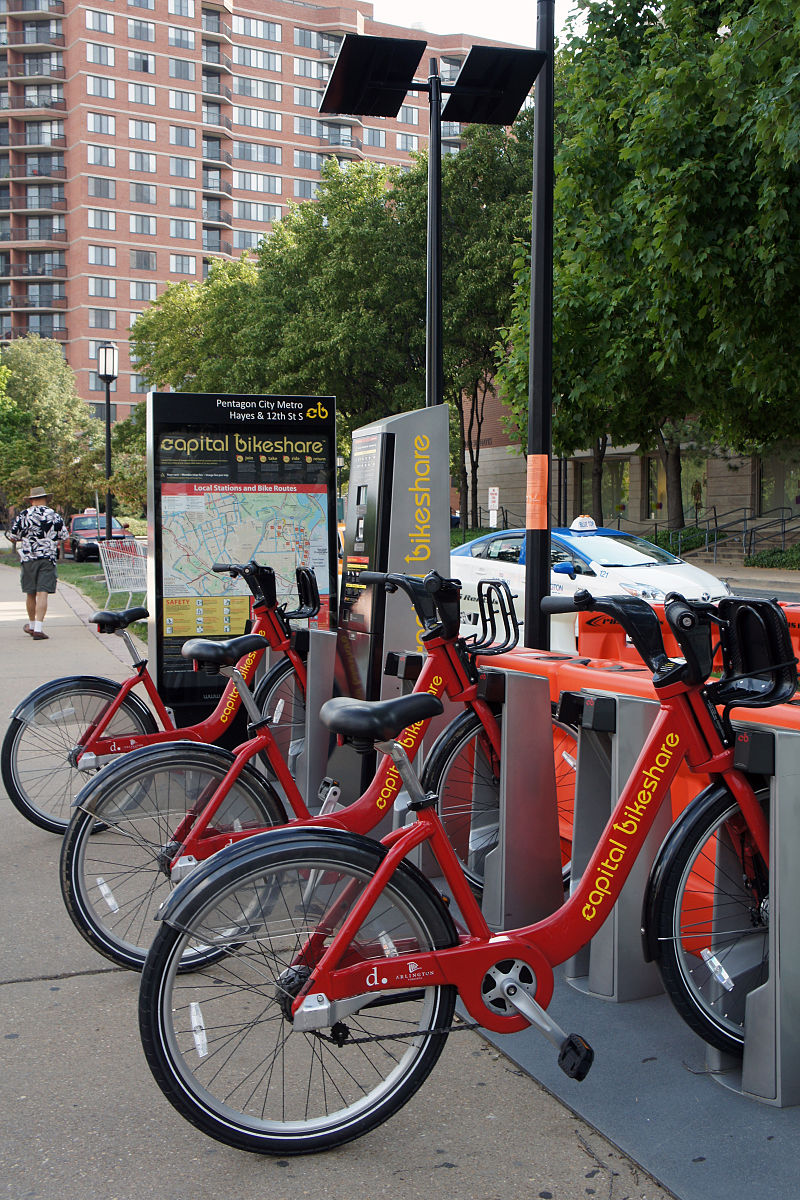
\includegraphics[]{800px-VA_07_2012_Capital_Bikeshare_4152.JPG}
            % \caption{By Mariordo (Mario Roberto Durán Ortiz) - Own work, CC BY-SA 3.0, https://commons.wikimedia.org/w/index.php?curid=20462784}
        \end{figure}
        \column{0.5\textwidth}
        \begin{itemize}
            \item Memberships are available for \$95 a year for unlimited trips under 45 minutes \cite{cabisite}. Casual users can pay \$1 to unlock the bike, then \$0.05 per minute.
            \item Primarily intended for short trips
            \item Docked bikeshare
            \item 700+ docks, ~35 million trips (so far)
        \end{itemize}

    \end{columns}
    \small{* recently, non-docked E-bikes that have been introduced}
\end{frame}

\begin{frame}
    \frametitle{The data}

    Capital Bikeshare publishes the following data about each trip on a monthly basis:

    \begin{itemize}
        \item start time
        \item end time
        \item start station index
        \item end station index
        \item Membership status of the rider (Member or Non-member?)
    \end{itemize}

    These data are available as csv files per month or year from Capital Bikeshare at https://ride.capitalbikeshare.com/system-data
\end{frame}

\begin{frame}
    \frametitle{My goal}


\end{frame}

\section{Methodology}
\begin{frame}
    \frametitle{Removing invalid trips}
    % sankey diagram?
    \section{What makes a trip invalid?}

    Longer than a 4 hours

    This is an arbitrary threshold. However, the CaBi system is primarily intended for short trips, and the pricing reflects this. The bikes can be used for leisure and tourism, but they are priced to encourage users to change bikes regularly. Also, for the purposes of this project, long trips are less likely to have


    Starting and ending at the same station

    For obvious reasons, cannot easily be routed

    Stations with an invalid start or end station

    A number of trips in the dataset are missing a value for the start or ending point

\end{frame}

\begin{frame}
    \frametitle{Find unique trips between two stations}

\end{frame}

\begin{frame}
    \frametitle{Building a Valhalla Routing network}

    \begin{itemize}
        \item Download OSM tiles
        \item Build Valhalla routing network
        \item Use Pandas the start and end point of every unique trip
    \end{itemize}
\end{frame}

\begin{frame}
    \frametitle{Build PostGIS topology at the same time}
    \begin{itemize}
        \item Using PLpgSQL triggers, add a corresponding entry to the topogeometry table for every new entry to the routes tables
    \end{itemize}
\end{frame}

\begin{frame}
    \frametitle{Sum up the trips on every topological element}

    
\begin{itemize}
    \item Using an SQL query, we can sum the trips on every unique street 
\end{itemize}

\end{frame}
\end{document}
